\chapter{Logistische Regression}
Dieses Kapitel befasst sich mit der Logistischen Regression. Zunächst wird die Definition und Funktion der Logistischen Regression erklärt. Danach wird die Geschichte und Entwicklung der Methode erörtert. Des weiteren gibt es eine Vertiefung der verschiedenen Regularisierungsmethoden und zum Abschluss die Grenzen der Funktion sowie einen Ausblick auf verwandte Algorithmen.
\section{Definition und Funktion}
Die logistische Regression ist ein statistisches Analyseverfahren, bei dem es darum geht, eine Beziehung zwischen einer abhängigen und mehrerer unabhängiger Variablen zu modellieren und wird auch als als binäres Logit-Modell bezeichnet.
Sie unterscheidet sich in soweit von der linearen Regression, dass die Voraussagen nicht spezielle Werte, sondern die Wahrscheinlichkeiten angeben, mit denen die jeweilige Ausprägung der Variable angenommen wird.\cite{ROHR} Die beiden Ausprägungen der abhängigen Variablen wird mit 0 bzw. 1 beschrieben, sodass die Vorhersage des Modells die Wahrscheinlichkeit beschreibt, mit der die abhängige Variable den Wert 1 annimmt, formal $P(Y_i=1)$ . Die Logistische Regression gehört zur Klasse der strukturen-prüfenden Verfahren und bildet eine Variation der Regressionsanalyse. Sie grenzt sich durch die Art ihrer abhängigen Variable, bezeichnet mit Y, welche als kategoriale Variable klassifiziert ist, von anderen Regressionsanalysen ab. Die Ausprägungen der Variable repräsentieren die verschiedenen Alternativen, in unserem binären (oder auch dichotomen) Fall ist "`trifft zu"' und "`trifft nicht zu"'.\cite{BECK}
Diese Gruppen werden nun mit 0 und 1 bezeichnet und für die Y Variable gilt nun: 
\begin{displaymath}
P(Y=0)=1-P(Y=1)\text{ und } P(Y=1)=1-P(Y=0)
\end{displaymath}
Ziel der Logistischen Regression ist es, gegeben Trainingsdaten 
$D = \{(X_1, y_1), \dots, (X_N,y_N)\}$ mit $X_i \in \mathbb R^d$ und $y_i \in 
\{0,1\}$ , ein Modell $f_{\beta}(x)$ für Vorhersagen finden, 
welches auf neuen, ungesehenen Daten einen möglichst kleinen Fehler macht.
Ausdrücken lässt sich das logistische Regressionsmodell nun wie folgt:
\begin{displaymath}
\pi(x) = f_{\beta}(x_{1},..,x_{n})
\end{displaymath}
Wobei $\pi(X_i)=P(Y=1|X_i)$ die bedingte Wahrscheinlichkeit, unter der das Ereignis 1 ("`trift zu"') mit den gegebenen Werten $X_i = (x_{i1},...,x_{id})^{T}$ eintritt, angibt.\\
Wie auch bei der Linearen Regression werden hierbei die unabhängigen Variablen linear miteinander kombiniert. Die sogenannte systematische Komponente des Modells wird durch die Linearkombination
\begin{displaymath}
z(X_i)=\beta_0 + \sum_{j=1}^{d}{\beta_j * x_{ij}} + u_i
\end{displaymath}
beschrieben. $\beta$ stellt hier den Vektor der Koeffizienten $(\beta_1 ,..., \beta_d)^T$ dar und $\beta_0$ ist der Bias. $u_i$ ist ein zu vernachlässigender Störterm.\cite{ROHR}
Um das Modell auszugestalten wird hier die logistische Funktion 
\begin{displaymath}
p=\dfrac{\exp(x)}{1+\exp(x)}=\dfrac{1}{1+\exp(-x)}
\end{displaymath}
verwendet.\cite{BECK}
In Abbildung 3.1 sieht man den s-förmigen Verlauf der Funktion. Dieser Verlauf, als Verteilungsfunktion interpretiert, approximiert die Verteilungsfunktion der Normalverteilung mit ausreichender Genauigkeit. Somit kann sie verwendet werden um reellwertige Variablen (im Wertebereich $[-\infty, +\infty]$) auf eine Wahrscheinlichkeit (im Wertebereich $[0,1]$) zu transformieren, denn die Verteilungsfunktion der Normalverteilung ist nur als Integral auszudrücken und damit schwer zu berechnen.\cite{WIKI}\cite{BECK}
\begin{figure}[ht]
\centering
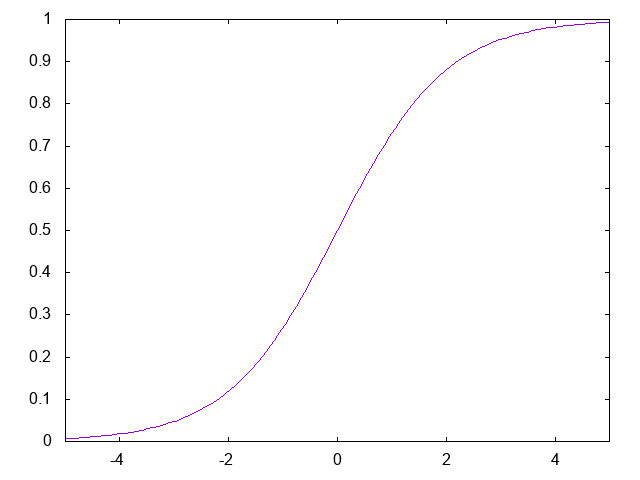
\includegraphics[scale=0.65]{bilder/logistic_reg_func}
\caption{Die logistische Funktion $p=\dfrac{1}{1+\exp(-x)}$ }
\end{figure}
\newpage
Wenn man diese Transformation der systematischen Komponente nun mit der logistischen Funktion durchführt erhält man die logistische Regressionsfunktion:
\begin{displaymath}
\pi(X)= \dfrac{1}{1+\exp(z(X))}
\end{displaymath}
Also genauer:
\begin{displaymath}
P(Y=1 | X=x_i)=P(Y_i=1)=\frac{\exp(\beta_0+x_i^T\beta)}{1+\exp(\beta_0+x_i^T\beta)} = \frac{1}{1+\exp(-(\beta_0+x_i^T\beta))}
\end{displaymath}
Die systemische Komponente $z(X)=\beta_0 + x_i^T\beta$ ist ein Prädiktor für $\pi(X)$. Je größer $z(X)$, desto größer auch $\pi(X)$ und damit auch $P(Y=1|X)$.\cite{BECK} 
\section{Lernen mit Logistischer Regression}
Die Anpassung der Koeffizienten erfolgt durch Minimierung der Loss Funktion: \begin{displaymath}
\min_\beta \sum_{i}^N \log(1+\exp(-(\beta_0+x_i^T\beta))) +C*R(\beta)
\end{displaymath}
Wobei $C \in \mathbb R$ ein Hyperparameter ist,der fest gewählt werden muss. Dies geschieht zumeist durch das Testen verschiedener Werte, sodass hier ein Ansatz zur Parallelisierung entsteht.
\section{Regularisierungsmethoden}
\subsection{LASSO}
L1-Regularisierung (Least Absolute Shrinkage and Selection Operator, kurz \textbf{LASSO}) mit $R(\beta) = \sum_{i}^N|\beta_i|$
\subsection{Ridge Regression}
L2-Regularisierung (Ridge Regression) mit $R(\beta)= \sum_{i}^N \beta_i^2$.
\section{Verwandte Algorithmen}